\documentclass[default]{beamer}
\setbeamertemplate{navigation symbols}{}

\usetheme{CambridgeUS}
%\useoutertheme{infolines}
\usecolortheme{beaver}

\usepackage[utf8]{inputenc}					% Выбор языка и кодировки
\usepackage[english, russian]{babel}	% Языки: русский, английский
\usepackage{csquotes}
\usepackage{tikz}
\usetikzlibrary{arrows,shapes,calc}
\usepackage{animate}
\usepackage{fp}
\usepackage{textpos}

\usepackage[
	language=auto,
	autolang=other,
	backend=biber,
	style=authortitle,
	sorting=ydnt,
	maxbibnames=5
]{biblatex}
\addbibresource{panov_mipt.bib}
				
\DeclareSourcemap{
	\maps[datatype=bibtex, overwrite]{
		\map{
			\step[fieldset=langid, fieldvalue=english]
			\step[fieldset=doi, null]
			\step[fieldset=issn, null]
			\step[fieldset=isbn, null]
			\step[fieldset=url, null]
			\step[fieldsource=language, fieldset=langid, origfieldval]
		}
	}
}
\DeclareBibliographyDriver{std}{%
	\usebibmacro{bibindex}%
	\usebibmacro{begentry}%
	\usebibmacro{author/editor+others/translator+others}%
	\setunit{\labelnamepunct}\newblock
	\usebibmacro{title}%
	\newunit\newblock
	\usebibmacro{maintitle+booktitle}
	\newunit\newblock
	\usebibmacro{journal}%
	\newunit\newblock
	\usebibmacro{date}%
	\newunit\newblock
	\usebibmacro{finentry}
}
\DeclareBibliographyAlias{article}{std}
\DeclareBibliographyAlias{book}{std}
\DeclareBibliographyAlias{inproceedings}{std}
\DeclareBibliographyAlias{incollection}{std}

\graphicspath{{../../images/}} 			% Пути к изображениям

\makeatletter
\setbeamertemplate{footline}
{
	\leavevmode%
	\hbox{%
		\begin{beamercolorbox}[wd=.333333\paperwidth,ht=2.25ex,dp=1ex,center]{author
				in head/foot}%
			\usebeamerfont{author in
				head/foot}\insertshortauthor~~\beamer@ifempty{\insertshortinstitute}{}{(\insertshortinstitute)}
		\end{beamercolorbox}%
		\begin{beamercolorbox}[wd=.333333\paperwidth,ht=2.25ex,dp=1ex,center]{title in
				head/foot}%
			\usebeamerfont{title in head/foot}\insertshorttitle
		\end{beamercolorbox}%
		\begin{beamercolorbox}[wd=.333333\paperwidth,ht=2.25ex,dp=1ex,right]{date in
				head/foot}%
			\usebeamerfont{date in head/foot}\insertshortdate{}\hspace*{1em}
			\insertframenumber{}\hspace*{2ex} 
		\end{beamercolorbox}
	}%
	\vskip0pt%
}

\addtobeamertemplate{frametitle}{}{
	\begin{textblock*}{100mm}(\textwidth-35pt,-20pt)
		
\includegraphics[width=1.5cm]{misc/logos/frccsc.png}
	\end{textblock*}
}

\newcommand{\predmatr}[3]{
	\node[ell, rectangle, minimum height = 15, minimum width = 7.5]  at (#1 pt,#2 pt) {}; 
	\node[ellf, rectangle, minimum height = 15, minimum width = 7.5] at (#1+7.5 pt,#2 pt) {};
	\node[minimum height = 15, minimum width = 15] (#3) at (#1+3.3pt,#2 pt) {};
	\draw[ell] (#1+7.5 pt,#2+7.5 pt) -- (#1 +7.5 pt,#2-7.5 pt);
}
\renewcommand*{\bibfont}{\tiny}
\setlength\bibitemsep{-5pt}

\begin{document}
	
	\title[Психология и ИИ]{Когнитивное компьютерное моделирование и искусственный интеллект}
	\author[Панов]{Александр Панов}
	\institute[ФИЦ ИУ РАН]{Отдел <<Интеллектуальные динамические системы и когнитивные исследования>>\\Институт системного анализа\\ Федеральный исследовательский центр <<Информатика и управление>>\\Российской академии наук}
	\date{19 марта -- Семинар AI@MIPT} 
	
	\begin{frame}
		\titlepage
		\centering
		\includegraphics[width=100pt]{misc/logos/ras.png} \hspace{10pt}
		
\includegraphics[width=80pt]{misc/logos/frccsc.png} \hspace{10pt}
		
\includegraphics[width=20pt]{misc/logos/hse.png}
	\end{frame}
	
	\begin{frame}
		\small
		\tableofcontents
	\end{frame}

	\section{Введение}
	\subsection{О лаборатории}
	
		
	\begin{frame}
		\frametitle{ФИЦ ИУ РАН}
		\begin{center}
			
\includegraphics[width=0.35\textwidth]{misc/logos/frccsc.png}
		\end{center}
		
		\par\bigskip
		\scriptsize
		Федеральный исследовательский центр <<Информатика и управление>> Российской Академии Наук "--- ведущая организация Российской Федерации, специализирующаяся в научных исследованиях в области информатики и управления.
		
		\textbf{Структурные подразделения:}
		\begin{itemize}
			\item Институт проблем информатики РАН (большие данные, информационная безопасность).
			\item Вычислительный центр РАН (машинное обучение, математическое моделирование).
			\item Институт системного анализа РАН (искусственный интеллект, системный анализ в экономике).
		\end{itemize}
		
		\textbf{Базовые кафедры:}
		\begin{itemize}
			\item ФУПМ МФТИ (<<Системные исследования»>> и <<Интеллектуальные системы>>).
			\item ВМК МГУ (<<Информационной безопасности>>).
			\item МГТУ, МИРЭА, МАИ.
		\end{itemize}
	\end{frame}

	\begin{frame}
		\frametitle{Отдел <<Интеллектуальные динамические системы и когнитивные исследования>>}
		
		\begin{columns}
			\begin{column}{0.7\textwidth}
				Основные направления исследований:
				\begin{itemize}
					\item Искусственный интеллект.
					\item Информационный поиск и анализ текстов (компьютерная лингвистика, психолингвистика, текстовая аналитика).
					\item Системы принятия решений (мультиможножества).
					\item Медицинские экспертные системы.
					\item Робототехнические системы (управление, обучение, планирование).
					\item Компьютерное когнитивные моделирование (модели когнитивных функций, многоагентные системы).
				\end{itemize}
				\par\bigskip
				45 научных сотрудников и инженерных специалистов, 4 доктора наук, 16 кандидатов наук.
			\end{column}
			\begin{column}{0.3\textwidth}
				\centering
				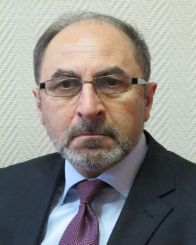
\includegraphics[width=0.4\textwidth]{misc/photos/gs}
				\par\smallskip
				\tiny
				Осипов Геннадий Семенович, зам. дир. ФИЦ ИУ РАН, проф., д.ф.-м.н., президент Российской ассоциации искусственного интеллекта (РААИ)
				\par\medskip
				
\includegraphics[width=0.4\textwidth]{misc/logos/exactus_logo.png}
				\par\medskip
				
\includegraphics[width=0.4\textwidth]{misc/logos/logo_like.png}
				\par\medskip
				
\includegraphics[width=0.4\textwidth]{misc/logos/logo_patent.png}

			\end{column}
		\end{columns}
	\end{frame}

	\begin{frame}
		\frametitle{Группа когнитивного компьютерного\\моделирования}
		\small
		\begin{columns}
			\begin{column}{0.5\textwidth}
				\vspace{-10pt}
				\begin{itemize}
					\item \textbf{Осипов Геннадий Семенович, д.ф.-м.н.},
					\item \textbf{Чудова Наталья Владимировна, к.псих.н.},
					\item \textbf{Кузнецова Юлия Михайловна, к.псих.н.},
					\item \textbf{Панов Александр, к.ф.-м.н.},
					\item Киселев Глеб, асп. ИСА РАН,
					\item Скрыник Алексей, асп. ИСА РАН,
					\item Ковалев Алексей, асп. ВШЭ,
					\item студенты SLabAI.
				\end{itemize}
			\end{column}
			\begin{column}{0.5\textwidth}
				Основные направления исследований:
				\begin{itemize}
					\item Моделирование картины мира человека.
					\item Моделирование когнитивных функций человека с учетом психологических и нейрофизиологических данных.
					\item Планирование поведения и целеполагание.
					\item Обучение и логический вывод в картине мира.
					\item Групповое и коалиционное поведение, распределение ролей.
				\end{itemize}
			\end{column}
		\end{columns}		
	\end{frame}	
	
	\begin{frame}
		\frametitle{Кратко о себе}
		\scriptsize
		\begin{columns}
			\begin{column}{0.85\textwidth}
				\textbf{Панов Александр Игоревич, к. ф.-м. н.}
				\begin{itemize}
					\item Выпускник НГУ и МФТИ.
					\item Старший научный сотрудник отдела <<Интеллектуальные динамические системы и когнитивные исследования>> ФИЦ ИУ РАН.
					\item Научный сотрудник и доцент ФКН ВШЭ.
					\item Доцент кафедры системных исследований Московского физико-технического института (МФТИ).
					\item Член Российской ассоциации искусственного интеллекта (РААИ).
					\item Член Сообщества биологически инспирированных когнитивных архитектур (BICA Society).
					\item Участие в организации Международной конференции по биологически инспирированным когнитивным архитектурам (BICA-2016 --- Нью-Йорк, BICA-2017 --- Москва), Международной школы по биологически инспирированным когнитивным архитектурам (Fierces on BICA, Москва) и школы молодых ученых по ИИ (ISyT 2017, Санкт-Петербург).
					\item Член редколлегии журнала Biologically Inspired Cognitive Architectures.					
					\item Руководитель проектов РФФИ мол\_а, мол\_а\_дк, офи\_м.
					\item Лауреат медали РАН для молодых ученых за 2017 год.
					\item Ментор студенческой лаборатории по ИИ (SLabAI).
				\end{itemize}
			\end{column}
			
			\begin{column}{0.15\textwidth}
				\centering
				\includegraphics[width=\textwidth]{misc/logos/ras.png}
				\vspace{7pt}
				
\includegraphics[width=\textwidth]{misc/logos/frccsc.png}
				\vspace{7pt}
				\includegraphics[width=0.7\textwidth]{misc/logos/isa.png}
				\vspace{7pt}
				\includegraphics[width=0.5\textwidth]{misc/logos/raai.png}
				\vspace{7pt}
				
\includegraphics[width=0.5\textwidth]{misc/logos/hse.png}
				\vspace{7pt}
				\includegraphics[width=\textwidth]{misc/logos/mipt.jpg}
				\vspace{5pt}
				\includegraphics[width=\textwidth]{misc/logos/BICA.png}
				\vspace{5pt}
				\includegraphics[width=0.7\textwidth]{misc/logos/slabai3.png}
			\end{column}
			
		\end{columns}
	\end{frame}
		
	\subsection{Психологические идеи}	
	\begin{frame}
		\frametitle{Когнитивные науки}

		\begin{center}
			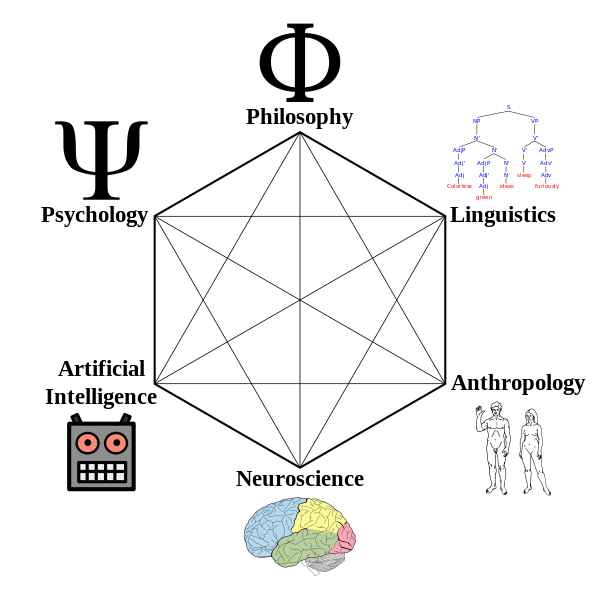
\includegraphics[width=0.3\textwidth]{cogsci.png}
		\end{center}
		
		Когнитивная наука (лат. cognitio <<познание>>) - междисциплинарное научное направление изучающее психику, разум (mind) человека и реализующие его процессы.
		\par\medskip
		Схожие направления в Европе и Америке: \textbf{Artificial General Intelligence} и \textbf{Сommon model of cognition}.
	\end{frame}

	\begin{frame}
		\frametitle{Проблема привязки символов}
		
		\begin{center}
			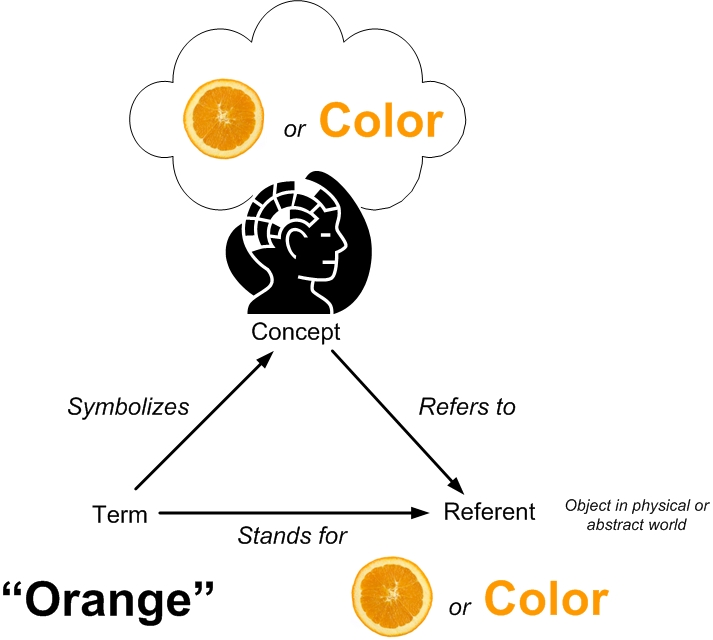
\includegraphics[width=0.3\textwidth]{symb_ground.jpg}
		\end{center}
		\scriptsize
		В оригинале Harnad "--- \textbf{symbol grounding problem} в 1990 г. 
		\par\medskip
		Классические методы искусственного интеллекта являются символьными (логика, множества правил, планирование, обучение). Однако, мышление "--- это больше, чем манипулирование символами.
		\par\medskip
		Особенно эта проблема актуальна в робототехнике (\textbf{symbol anchoring}) "--- система должна обучаться символам на основе своего собственного опыта.
		\nocite{*}
		\printbibliography[keyword={sgp}, resetnumbers=true]
	\end{frame}

	\begin{frame}
		\frametitle{Нейросимвольные вычисления}
		
		\begin{center}
			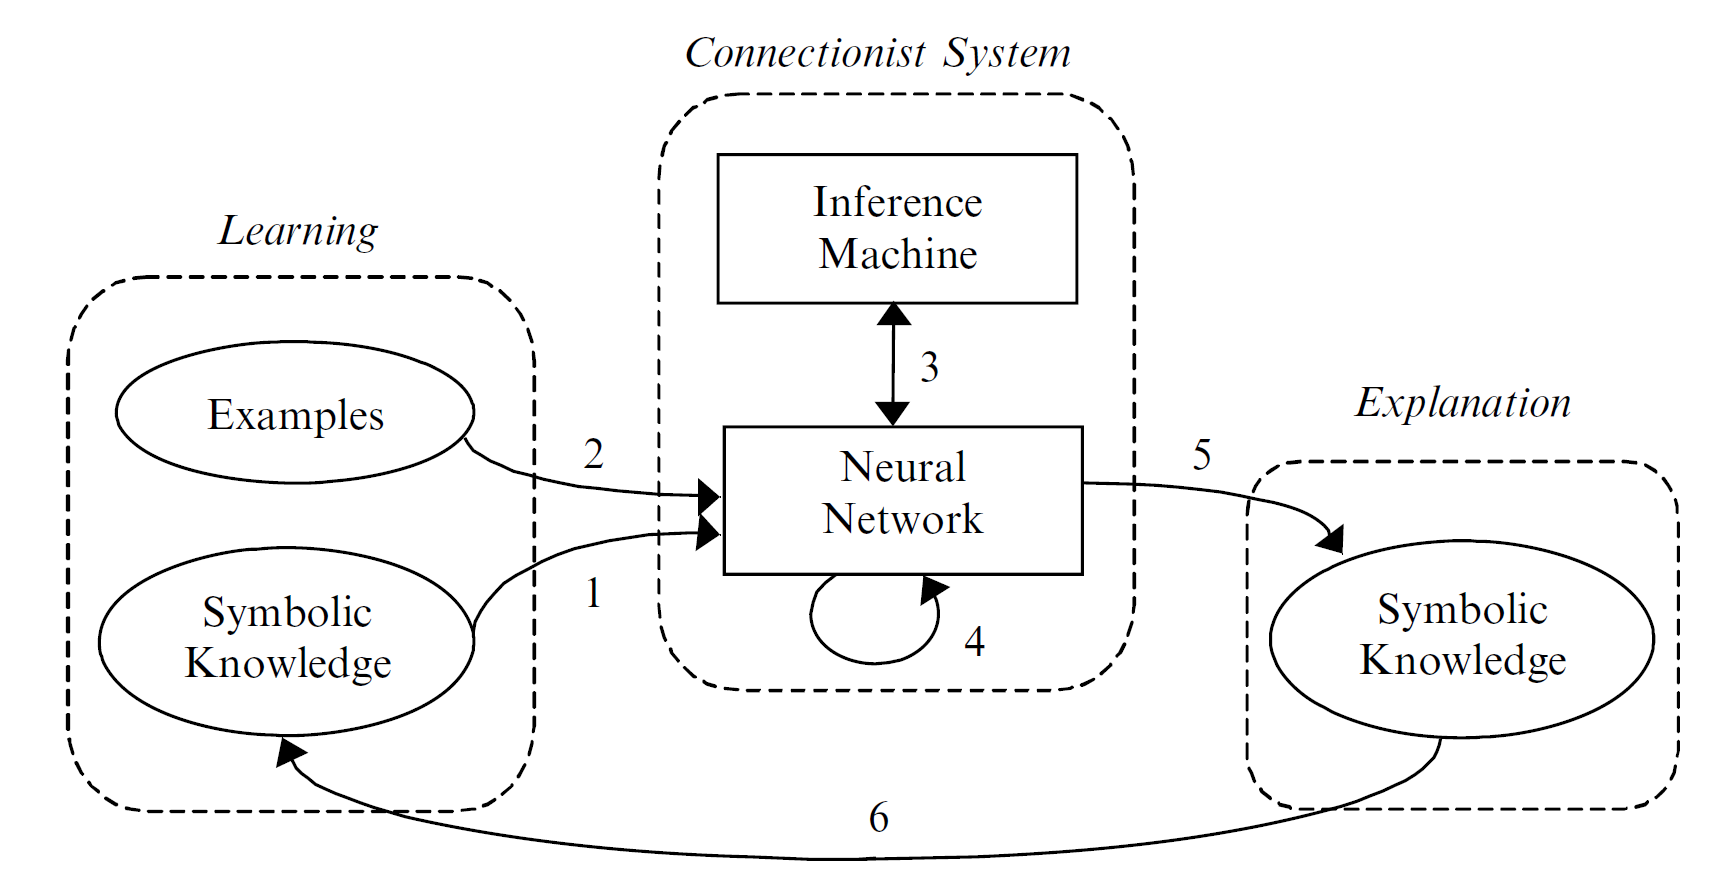
\includegraphics[width=0.3\textwidth]{neuro_symb.png}
		\end{center}
		\textbf{Основная идея}: кодирование символа путем вектора чисел и затем представление этого вектора с помощью связей в ансамбле искусственных нейронов (embending).
		\par\medskip
		\textbf{Основной результат}: путем введения специальных правил по распространению активности по нейронной сети реализованы некоторые простые логические схемы.
		\par\medskip
		\textbf{Основной недостаток}: ограниченная интеграция обучения.
		\nocite{*}
		\printbibliography[keyword={neuro_symb}, resetnumbers=true]
	\end{frame}

	\begin{frame}
		\frametitle{Знак vs. символ}
		\onslide<1->{
		Если прямая интеграция нейронных сетей и символьной обработки работает плохо, то возможно стоит пересмотреть роль \textbf{символа} в общей схеме?
		\par\medskip
		Будем считать, что у символа есть своя структура и у него есть кроме \textbf{номитативной} и другие \textbf{функциональные} роли в реализации когнитивных процессов $\rightarrow$ \textbf{знак}.
		\par\medskip
		Понятие знака как элемента индивидуального знания появилось в концк XIX в.: Пирс, Фреге. Нашло свое отражение в лингвистике, логике, культурологии и \textbf{психологии}.
		}
		\onslide<2->{
			\tikz[baseline]{
			\node[fill=blue!20, rounded corners=5pt, minimum width=330, minimum height = 40] (k1) {
				\begin{minipage}[t][40pt]{330pt}
					\textbf{Идея}: формализовать понятие знака $\rightarrow$ использовать знак в качестве основного структурного элемента системы знаний когнитивного агента $\rightarrow$ построить знаковые модели когнитивных функций.
				\end{minipage}
				
			};
			}
			
		}
		\onslide<1->{
		\vspace{-5pt}
		\nocite{*}
		\printbibliography[keyword={semiotics}, resetnumbers=true]
		}
	\end{frame}
	
	\begin{frame}
		\frametitle{Культурно-исторический подход Выготского}
		\begin{center}
			\includegraphics[width=0.15\textwidth]{misc/photos/vygotsky.jpg}
		\end{center}
		\scriptsize
		Теория происхождения и развития высших психических функций:
		\begin{itemize}
			\item \textbf{Социальная среда} "--- главный источник развития личности.
			\item Овладение культурой, способами поведения и мышления.
			\item Развитие когнитивных функций происходит в первую очередь через использование ребенком \textbf{<<психологических орудий>>}, путем овладения системой знаков-символов, таких как язык, письмо, счет.
			\item Внешняя деятельность, когда культурные средства имеют предметный вид, по мере отработки сворачивается (\textbf{интериоризуется}) во внутренний план.
			\item На первом этапе внешней деятельность ребенок все делает в \textbf{сотрудничестве} со взрослыми, <<зона ближайшего развития>>.
			\item Развитие - не ровно-постепенный, а \textbf{стадиальные} процесс.
			\item Сознание развивается через \textbf{диалог}: диалог ребенка со взрослым либо диалог взрослого со взрослым.
		\end{itemize}
		\end{frame}
		
		\begin{frame}
		\frametitle{Теория деятельности Леонтьева}
		\begin{columns}
		\begin{column}{0.4\textwidth}
			\includegraphics[width=0.8\textwidth]{misc/psycho/activity.pdf}			
		\end{column}
		\begin{column}{0.6\textwidth}
			\begin{center}
				\includegraphics[width=0.17\textwidth]{misc/photos/leontyev.jpg}
			\end{center}
			Основные положения:
			\begin{itemize}
				\item Поведение человека - это двойная иерархическая структура мотивы-цели и действия-операции.
				\item Деятельность – это активный, целенаправленный процесс.
				\item Действия человека предметны; их цели носят социальный характер.
				\item Сознание и деятельность неразрывно связаны.
			\end{itemize}
		\end{column}
		\end{columns}
	\end{frame}

	\begin{frame}
		\frametitle{Знак как орудие психической деятельности}
		\begin{center}
			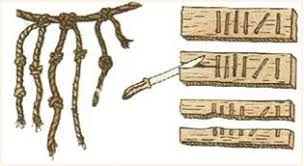
\includegraphics[width=0.4\textwidth]{link.jpg}
		\end{center}

		\begin{itemize}
			\item Знак - это искусственно созданный человеком стимул, средство для управления своим поведение и поведением других.
			\item История развития человечества - это история развития знака: чем более развита система знаков в поколении, тем более развиты высшие психические функции.
			\item Знаки: наскальный рисунок, приметы, жесты, речь, ноты и т.д.
		\end{itemize}
	\end{frame}

	\begin{frame}
		\frametitle{Прикладная семиотика}
		\begin{center}
			\includegraphics[width=0.2\textwidth]{signs/ru/sign-frame.png}
		\end{center}
		\vspace{-15pt}
		\scriptsize
		Семиотические базы знаний:
		\begin{itemize}
			\item \textbf{Именованность}: информационная единица, которая претендует на то, чтобы называться знанием, должна иметь некоторую собственную метку - имя.
			\item \textbf{Структурированность}: информационная единица должна обладать своей внутренней структурой.
			\item \textbf{Принцип матрешки}: знаки за счет связей наследования как бы вкладываются друг в друга, обеспечивая описание сущностей на различных уровнях.
			\item \textbf{Связность}: знаки благодаря различным отношениям объединяются в сеть.
			\item \textbf{Активность}: в сетях знаков становится возможной реализация принципа <<активизация знаний - источник активизации процедур>>.
			\item \textbf{Рефлексивность}: появление метауровня позволяет системе рассуждать о самой себе, о характере имеющейся у нее информации об окружающем мире.
		\end{itemize}
		\vspace{-5pt}
		\nocite{*}
		\printbibliography[keyword={apply}, resetnumbers=true]
	\end{frame}

	\begin{frame}
		\frametitle{Когнитивные архитектуры}
		\begin{center}
			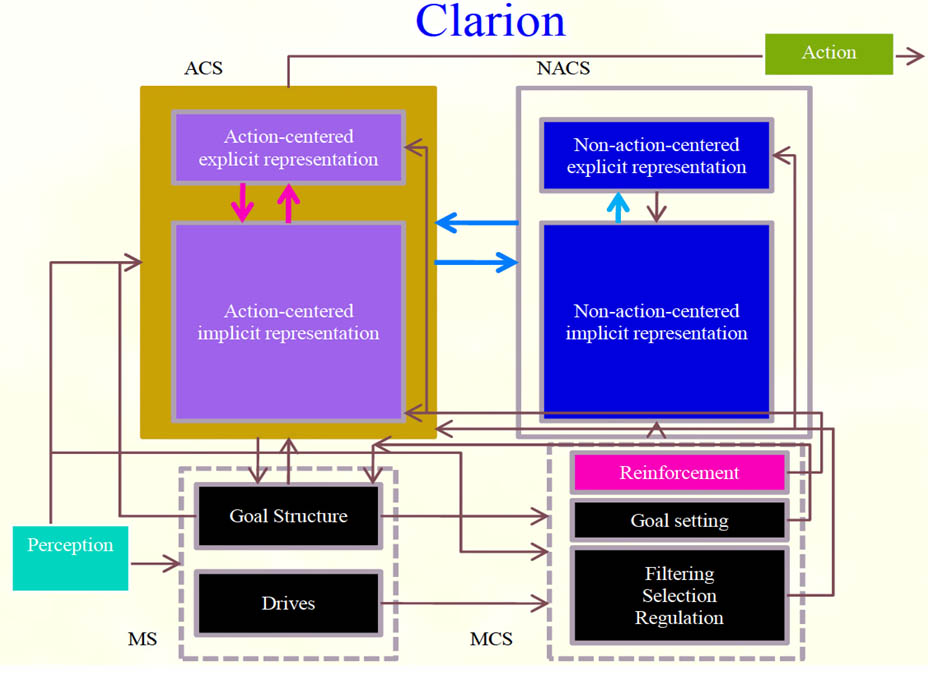
\includegraphics[width=0.3\textwidth]{clarion.jpg}
			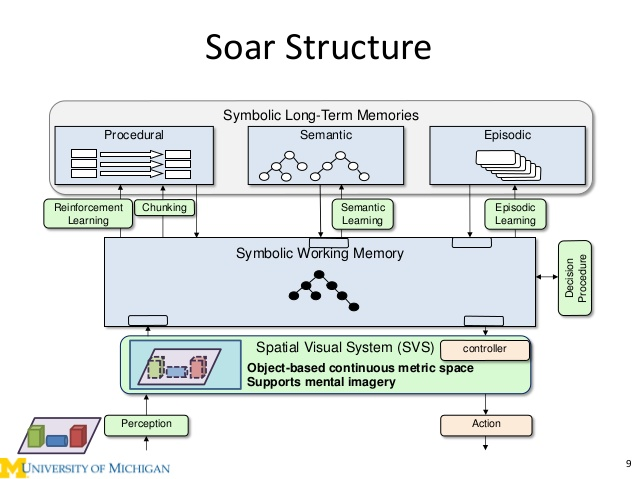
\includegraphics[width=0.3\textwidth]{soar.jpg}
		\end{center}
		\scriptsize
		Недостатки современных когнитивных архитектур:
		\begin{itemize}
			\item Концептуальная нерешенность проблемы привязки символов (symbol grounding problem) - CLARION
			\item Отсутствие деятельностной модели поведения системы - реализация только некоторых когнитивных аспектов
			\item Иерархичность представления знаний (4D/RCS)
			\item Возможность реализации иерархического планирования
			\item Реализация обучения концептуальным знаниям - Cognitive Mario
			\item Моделирование рефлексивного поведения
		\end{itemize}
		\vspace{-5pt}
		\nocite{*}
		\printbibliography[keyword={symbgrnd}, resetnumbers=true]
	\end{frame}

		\section{Модель элементов картины мира}
	\subsection{Знаковая картина мира}
	
	\begin{frame}
		\frametitle{Картина мира субъекта деятельности}
		\scriptsize
		\onslide<1->{
			Картина мира субъекта деятельности - это представления субъекта о внешней среде, о своих собственных характеристиках, целях, мотивах, о других субъектах и операции (произвольные и непроизвольные), осуществляемые на основе этих представлений.
		}
		\onslide<2->{
			\par\smallskip
			Элементом картины мира является знак:
			\begin{itemize}
				\item в смысле культурно-исторического подхода Выготского-Лурии,
				\item выполняющий функции в соответствии с теорией деятельности Леонтьева.
			\end{itemize}
		}
		\onslide<3->{
			\begin{columns}
				\begin{column}{0.4\textwidth}
					\centering
					\includegraphics[width=0.6\textwidth]{signs/ru/sign_color_book_ru}
				\end{column}
		}
		\onslide<4->{
				\begin{column}{0.6\textwidth}
					\begin{columns}
						\begin{column}{0.5\textwidth}
							\centering
							\includegraphics[width=\textwidth]{misc/phisio/ivan_cyrc}
						\end{column}
						\begin{column}{0.5\textwidth}
							\centering
							\includegraphics[width=\textwidth]{misc/phisio/workspace}
						\end{column}
					\end{columns}
					
				\end{column}
			\end{columns}
			В пользу существования такой структуры свидетельствуют:
			\begin{itemize}
				\item нейрофизиологические данные (Эдельман, Иваницкий, Маунткастл и др.),
				\item другие психологические теории (например, трехкомпонентная модель Станович).
			\end{itemize}
			\vspace{-5pt}
			\nocite{*}
			\printbibliography[keyword={sign}, resetnumbers=true]
		}
	\end{frame}
	
	\begin{frame}
		\frametitle{Три образующих элемента картины мира}
		\footnotesize
		\begin{figure}
			\includegraphics[width=0.3\textwidth]{signs/ru/sign_colored}
		\end{figure}
		
		Представляемая сущность описывается тремя причинно-следственными (каузальными) структурами:
		\begin{itemize}
			\item {\color{red}структура образа} - представление взаимосвязи внешних сигналов и внутренних характеристик субъекта (агента) - сенсо-моторное представление,
			\item {\color{blue}структура значения} - обобщенное знание о соотношениях во внешнем мире, согласованное в некоторой группе субъектов (агентов),
			\item {\color{green!60!black}структура личностного смысла} - ситуационная потребностно-мотивационная интерпретация знаний о соотношениях во внешней среде (значение для себя).
		\end{itemize}
	\nocite{*}
	\printbibliography[keyword={qualia}, resetnumbers=true]
	\end{frame}

	\begin{frame}
		\frametitle{Актуализация и формирование знака}
		\begin{figure}
			\includegraphics[width=0.4\textwidth]{signs/en/sign_naming_colored_en}
		\end{figure}
		\small
		\textbf{Процесс обучения} "--- образование новых знаков как неподвижная точка операторов замыкания $\Psi_p^m\Psi_m^a\Psi_a^p$.
		\par\smallskip
		Реализация когнитивных функций "--- \textbf{актуализация} (активация) имеющихся знаков и формирование новых <<ситуационных>> знаков "--- <<протознаков>> без конвенционального имени.
	\end{frame}

	\begin{frame}
		\frametitle{Уровни представления}
		\begin{figure}
			\includegraphics[width=0.7\textwidth]{signs/ru/sign_levels}
		\end{figure}
	\end{frame}

	\subsection{Нейронный субстрат}

	\begin{frame}
		\frametitle{Нейронный субстрат}
		
		\begin{columns}
			\begin{column}{0.35\textwidth}
				\includegraphics[width=0.8\textwidth]{misc/phisio/mozg_2}
				\par\bigskip
				\hspace{-7mm}\includegraphics[width=\textwidth]{misc/phisio/mozg}
			\end{column}
			\begin{column}{0.65\textwidth}
				\includegraphics[width=\textwidth]{misc/phisio/cortex_layers}
			\end{column}
		\end{columns}
		\nocite{*}
		\printbibliography[keyword={column}, resetnumbers=true]
	\end{frame}

	
	\begin{frame}
		\frametitle{Гетерархическая модель}
		\scriptsize
		Разработана расширенная реализация иерархической временной памяти (hierarchical temporal memory - HTM) - \textbf{гетерархическая каузальная сеть (heterarchical causal network - HCN)}.
		
		\begin{center}
			\includegraphics[width=0.4\textwidth]{misc/mpf/hawkins_htm}
		\end{center}
		\nocite{*}
		\printbibliography[keyword={starthtm}, resetnumbers=true]
	\end{frame}

	\begin{frame}
		\frametitle{Гетерархическая модель}

		\begin{center}
			\includegraphics[width=0.3\textwidth]{misc/mpf/hawkins_htm_ex_a}
			\includegraphics[width=0.3\textwidth]{misc/mpf/hawkins_htm_ex_b}
		\end{center}
		\nocite{*}
		\printbibliography[keyword={hetermem}, resetnumbers=true]
	\end{frame}
		
	\begin{frame}
		\frametitle{Нейронная организация}
		
		\begin{columns}
			\begin{column}{0.65\textwidth}
				\includegraphics[width=0.9\textwidth]{misc/mpf/regions_connect}
			\end{column}
			\begin{column}{0.35\textwidth}
				\includegraphics[width=\textwidth]{misc/phisio/column}
			\end{column}
		\end{columns}
		\nocite{*}
		\printbibliography[keyword={simplehtm}, resetnumbers=true]
	\end{frame}
	
	\begin{frame}
		\frametitle{Модель процесса обучения}
		
		К основным принципам работы механизма обучения относятся: 
		
		\begin{itemize}
			\item использование иерархии вычислительных узлов с восходящими и нисходящими связями, 
			\item использование Хэббовских правил обучения, 
			\item разделение пространственного и временного группировщиков, 
			\item подавление второстепенной активации для формирования разреженного представления.
		\end{itemize}
		
		В результате работы механизма обучения по прецедентам (без учителя) формируются так называемые \textbf{каузальные матрицы}.
		\vfill
		\nocite{*}
		\printbibliography[keyword={htmlearn}, resetnumbers=true]
	\end{frame}	
	
	\subsection{Образная компонента знака}
	\begin{frame}
		\frametitle{Каузальная матрица}                             
		\centering
		\includegraphics[width=0.7\textwidth]{causnet/caus_matr}
		\vspace{10pt}
		\nocite{*}
		\printbibliography[keyword={per}, resetnumbers=true]
	\end{frame}

	\begin{frame}
		\frametitle{Алгоритм $\mathfrak A_{th}$ активации образа знака}
		
		\begin{tikzpicture}[overlay,remember picture]
		
		\tikzstyle{z_matrix} = [draw, rectangle, minimum width = 60, minimum height = 60,fill=white];
		
		\onslide<1->{
			\node (meas_fun) at (0.7,0.5) {$\hat f_1,\hat f_2\dots,\hat f_k$};	
		}
		\onslide<2->{
			\node (control_vect) at ($(meas_fun)+(-0.5,1.2)$) {$\hat x^{j+1}$};
			\path[->,thick,red] (control_vect.east)  edge[out = -45, in = 45, right] (meas_fun.north); 
		}
		\onslide<3->{
			\node[z_matrix] (z_1) at ($(meas_fun)+(2.6,-0.5)$) {};
			\node[z_matrix] at ($(z_1)+(0.2,-0.1)$) {};
			\node[z_matrix] at ($(z_1)+(0.4,-0.2)$) {};
			
			\node[z_matrix] at ($(z_1)+(0.9,-0.5)$) {};
			\node[z_matrix] at ($(z_1)+(1.1,-0.6)$) {};
			\node[z_matrix] at ($(z_1)+(1.3,-0.7)$) {};
			
			\path[->,thick,blue] ([xshift=20]meas_fun.south)  edge[out = -90, in = -155, right] ($(z_1)+(-1,-1.2)$);
			\path[->,thick,blue] ([xshift=-25]meas_fun.south)  edge[out = -90, in = -155, right] ($(z_1)+(-0.1,-1.7)$);
			
			\node at ($(z_1)+(-1,1.4)$) {$Z^*$};
			
			\node at ($(z_1)+(0.8,1.4)$) {$Z_1$};
			\node at ($(z_1)+(1.4,1.2)$) {$\ddots$};
			\node at ($(z_1)+(2,0.9)$) {$Z_k$};
		}
		
		\onslide<4->{
			\draw[ultra thick, green!60!black] ($(z_1)+(-0.4,-1.1)$) -- ($(z_1)+(-0.4,0.6)$);
			\draw[ultra thick, green!60!black] ($(z_1)+(0.5,-1.6)$) -- node[right,black] {$z_1^r$} ($(z_1)+(0.5,0.1)$);
			
			\draw[->, thick, green!60!black] ($(z_1)+(-0.1,-3)$) -- node[right,black] {$\bar x(0)$} ($(z_1)+(-0.1,-2)$);
		}
		
		\onslide<5->{
			\node[z_matrix] (z_2) at ($(z_1)+(5,0)$) {};
			\node[z_matrix] at ($(z_2)+(0.2,-0.1)$) {};
			
			\node[z_matrix] at ($(z_2)+(0.9,-0.5)$) {};
			\node[z_matrix] at ($(z_2)+(1.3,-0.7)$) {};
			
			\node at ($(z_2)+(-1,1.4)$) {$Z^*$};
			\node at ($(z_2)+(0.8,1.4)$) {$Z_1$};
			\node at ($(z_2)+(1.4,1.2)$) {$\ddots$};
			\node at ($(z_2)+(2,0.9)$) {$Z_k$};
			
			\draw[->, ultra thick] ($(z_1)+(2.6,-0.6)$) -- node [above] {\scriptsize$\frac{\|\bar z_1^r-\bar x(0)\|}{\|\bar z_1^r\|+\|\bar x(0)\|}$} ($(z_1)+(3.7,-0.6)$);
			
			\draw[ultra thick, dotted, green!60!black] ($(z_2)+(-0.6,-1)$) -- ($(z_2)+(-0.6,0.7)$);
			\draw[ultra thick, dotted, green!60!black] ($(z_2)+(0.5,-1.6)$) -- ($(z_2)+(0.5,0.1)$);
		}
		
		\onslide<6->{
			\draw[->, thick, red] ($(z_2)+(0.3,1.4)$) -- node[right,black] {$\bar x^*(0)$} ($(z_2)+(0.3,3)$);
		}
		
		\onslide<7>{
			\draw[<-, thick, red] ($(z_2)+(-0.1,-3)$) -- node[right,black] {$\hat x^j(0)$} ($(z_2)+(-0.1,-2)$);
		}
		
		\onslide<7->{				
			\draw[ultra thick, green!60!black] ($(z_2)+(-0.4,-1)$) -- ($(z_2)+(-0.4,0.7)$);
			\draw[ultra thick, green!60!black] ($(z_2)+(0.7,-1.6)$) -- node[right,black] {$z_2^r$} ($(z_2)+(0.7,0.1)$);	
		}
		\onslide<8->{
			\draw[->, thick, green!60!black] ($(z_2)+(-0.1,-3)$) -- node[right,black] {$\bar x(1)$} ($(z_2)+(-0.1,-2)$);
		}
		
		\onslide<9->{
			\draw[->, ultra thick] ($(z_2)+(2.6,-0.6)$) -- node [above] {\scriptsize$\frac{\|\bar z_1^r-\bar x(1)\|}{\|\bar z_1^r\|+\|\bar x(1)\|}$} ($(z_2)+(3.7,-0.6)$);
		}
		\end{tikzpicture}
		
	\end{frame}	

	\subsection{Каузальная сеть}
	\begin{frame}
		\frametitle{Каузальная сеть на образах}
		\footnotesize
		\textbf{Каузальная сеть} на множестве образов знаков $W_p=\langle V_p, E_p \rangle$ - помеченный ориентированный граф, в котором
		\begin{itemize}
			\item каждому узлу $v\in V_p$ ставится в соответствие кортеж казуальных матриц $Z^p(s)$ образа некоторого знака $s$ ($v\rightarrow Z^p(s)$);
			\item ребро $e=(v_1, v_2)$ принадлежит множеству ребер графа $E$, если $v_1\rightarrow Z^p(s_1), v_2\rightarrow Z^p(s_2)$ и $s_1\in S_p(s_2)$;
			\item каждому ребру графа $e=(v_1, v_2), v_1\rightarrow Z^p(s_1), v_2\rightarrow Z^p(s_2)$ ставится в соответствие метка $\epsilon=(\epsilon_1,\epsilon_2,\epsilon_3)$ - кортеж трех натуральных чисел:
			\begin{itemize}
				\item $\epsilon_1$ - индекс исходной матрицы в кортеже $Z^p(s_1)$, может принимать специальное значение 0, если исходными могут служить любые матрицы из кортежа;
				\item $\epsilon_2$ - индекс целевой матрицы в кортеже $Z^p(s_2)$, строка которой ставится в соответствие признаку $s_1$;
				\item $\epsilon_2$ - индекс столбца в целевой матрице, в которой в соответствующей признаку $s_1$ строке стоит 1, может принимать положительные значения (\textit{столбцы условий}) и отрицательные (\textit{столбцы эффектов}).
			\end{itemize}		
		\end{itemize}
	\end{frame}

	\begin{frame}
		\frametitle{Каузальная сеть на образах: пример}
		
		\centering
		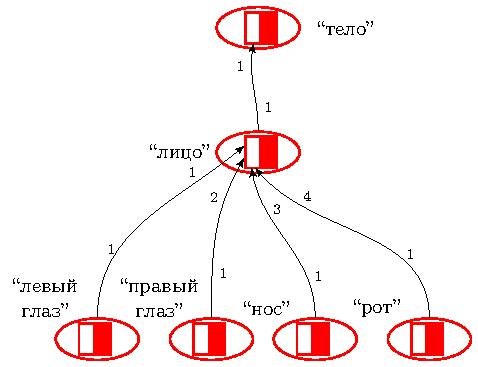
\includegraphics[page=1,width=0.6\textwidth]{examples/causnet/caus_net_colored}
		\includegraphics[width=0.4\textwidth]{misc/photos/face}
	
		\nocite{*}
		\printbibliography[keyword={signopernew}, resetnumbers=true]
	\end{frame}

	\begin{frame}
		\frametitle{Каузальная сеть на значениях: пример}
		
		\begin{figure}
			\includegraphics[page=2,width=0.7\textwidth]{examples/causnet/caus_net_colored}
		\end{figure}
		
	\end{frame}

	\begin{frame}
		\frametitle{Каузальная сеть на личностных смыслах: пример}
		
		\begin{figure}
			\includegraphics[page=3,width=0.7\textwidth]{examples/causnet/caus_net_colored}
		\end{figure}
		
	\end{frame}	

	\subsection{Семиотическая сеть}

	\begin{frame}
		\frametitle{Картина мира субъекта деятельности}
		
		\begin{columns}
			\begin{column}{0.45\textwidth}
				\begin{figure}
					\includegraphics[width=\textwidth]{signnet/signs_net}
				\end{figure}
			\end{column}
			\begin{column}{0.55\textwidth}
				\scriptsize
				\textbf{Знаком} будем называть четверку $s=\langle n,p,m,a\rangle$, где $n$ - имя знака,  $p=Z^p, m=Z^m,a=Z^a$ - кортежи каузальных матриц, которые соответственно называются образом, значением и личностным смыслом знака $s$.
				\par\medskip
				\textbf{Семиотическая сеть} - пятерка $\Omega=\langle W_p, W_m, W_a, R_n, \Theta, \Phi\rangle$, где
				\begin{itemize}
					\item $W_p, W_m, W_a$ - соответственно каузальные сети на множестве образов, значений и личностных смыслах,
					\item $R_n$ - семейство отношений на множестве знаков, сгенерированных на основе трех каузальных сетей, т.е. $R_n=\{R_p, R_m, R_a\}$,
					\item $\Theta$ - семейство операций на множестве знаков,
					\item $\Theta$ - правила распространения активности на каузальных сетях.
				\end{itemize}
			\end{column}
		\end{columns}
		\nocite{*}
		\printbibliography[keyword={symbsign}, resetnumbers=true]
	\end{frame}	

	
		\section{Модели когнитивных функций}
	
	\begin{frame}
		\small
		\tableofcontents
	\end{frame}
	
	\begin{frame}
		\frametitle{Образование нового знака}
		\centering
		\includegraphics[width=0.5\textwidth]{signs/en/sign_naming_colored_en}
	\end{frame}		
	
	\begin{frame}
		\frametitle{Отношения на множестве компонент знака}
		\centering
		\includegraphics[page=1,width=0.8\textwidth]{sign-schemas/sign_relations}
		
		Сходство образов
	\end{frame}	
	
	\begin{frame}
		\frametitle{Отношения на множестве компонент знака}
		
		\begin{columns}
			\begin{column}{0.3\textwidth}
				\centering
				Включение образов 
				\par\bigskip
				\par\bigskip
				\par\bigskip
				\par\bigskip
				\par\bigskip
				Противопоставление образов 
				
			\end{column}
			\begin{column}{0.7\textwidth}
				\includegraphics[page=2,width=0.8\textwidth]{sign-schemas/sign_relations}
				
				\includegraphics[page=3,width=0.8\textwidth]{sign-schemas/sign_relations}
			\end{column}
		\end{columns}
		
	\end{frame}	
	
	\begin{frame}
		\frametitle{Отношения на множестве компонент знака}
		\centering
		\includegraphics[page=4,width=0.7\textwidth]{sign-schemas/sign_relations}
		
		Сценарий на значениях
	\end{frame}	
	
	\begin{frame}
		\frametitle{Отношения на множестве компонент знака}
		
		\begin{columns}
			\begin{column}{0.3\textwidth}
				\centering
				Поглощение личностных смыслов 
				\par\bigskip
				\par\bigskip
				\par\bigskip
				\par\bigskip
				\par\bigskip
				Противопоставление личностных смыслов 
				
			\end{column}
			\begin{column}{0.7\textwidth}
				\includegraphics[page=5,width=0.8\textwidth]{sign-schemas/sign_relations}
				\par\bigskip
				\includegraphics[page=6,width=0.8\textwidth]{sign-schemas/sign_relations}
			\end{column}
		\end{columns}
	\end{frame}	

	\subsection{Операции в семиотической сети}	

	\begin{frame}
		\frametitle{Операции на множестве компонент знака}
		
		\begin{columns}
			\begin{column}{0.5\textwidth}
				\centering
				\includegraphics[page=7,width=\textwidth]{sign-schemas/sign_relations}
				\par\bigskip
				Замыкание по значениям
			\end{column}
			\begin{column}{0.5\textwidth}
				\centering
				\includegraphics[page=8,width=\textwidth]{sign-schemas/sign_relations}
				\par\bigskip
				Агглютинация личностных смыслов
			\end{column}
		\end{columns}
		\nocite{*}
		\printbibliography[keyword={signoper}, resetnumbers=true]
	\end{frame}	
	
	\begin{frame}
		\frametitle{Модель функции планирование поведения}
		\centering
		\includegraphics[width=0.9\textwidth]{algo/ru/plan_alg_ru}
		\nocite{*}
		\printbibliography[keyword={signb}, resetnumbers=true]
		\nocite{*}
		\printbibliography[keyword={symbsign}, resetnumbers=true]
	\end{frame}	
	
	\subsection{Планирование поведения}
	\begin{frame}
		\frametitle{Алгоритм планирования поведения}
		
		\begin{columns}
			\begin{column}{0.6\textwidth}
				\includegraphics[width=\textwidth]{algo/ru/beh_plan2_ru}
				\vspace{10pt}
				\nocite{*}
				\printbibliography[keyword={plan}, resetnumbers=true]
				\printbibliography[keyword={causnet}]
			\end{column}
			\begin{column}{0.4\textwidth}
				\scriptsize
				Иерархический процесс планирования начинается с конченой ситуации и стремится достичь начальной ситуации.
				\par\bigskip
				MAP-итерация:
				\begin{itemize}
					\item \textit{S-step} -- поиск прецедентов выполнения действия в текущих условиях,
					\item \textit{M-step} -- поиск применимых действий на сети значений,
					\item \textit{A-step} -- генерация личностных смыслов, соответствующих найденным значениям,
					\item \textit{P-step} -- построение новой текущей ситуации по множеству признаков условий найденных действий.
					
				\end{itemize}
			\end{column}
		\end{columns}
		
	\end{frame}		
	
	\subsection{Примеры}
	\begin{frame}
		\frametitle{Пример: фрагмент сети на значениях}
		\begin{columns}
			\begin{column}{0.7\textwidth}
				\centering
				\includegraphics[page=2,width=\textwidth]{examples/plan/plan_nets}
			\end{column}
			\begin{column}{0.3\textwidth}
				\centering
				\includegraphics[page=1,width=\textwidth]{examples/plan/block_world}
			\end{column}
		\end{columns}
	\end{frame}	
	
	\begin{frame}
		\frametitle{Пример: сеть на смыслах - начальная ситуация}
		
		\centering
		\includegraphics[page=3,width=0.7\textwidth]{examples/plan/plan_nets}
		\par\bigskip
		\includegraphics[page=2,width=0.5\textwidth]{examples/plan/block_world}
		
		
	\end{frame}	
	
	\begin{frame}
		\frametitle{Пример: сеть на смыслах - целевая ситуация}
		\begin{columns}
			\begin{column}{0.7\textwidth}
				\centering
				\includegraphics[page=1,width=\textwidth]{examples/plan/plan_nets}
			\end{column}
			\begin{column}{0.3\textwidth}
				\centering
				\includegraphics[page=1,width=\textwidth]{examples/plan/block_world}
			\end{column}
		\end{columns}
	\end{frame}	
	
	\begin{frame}
		\frametitle{Пример: фрагмент сети на значениях}
		\begin{columns}
			\begin{column}{0.7\textwidth}
				\centering
				\includegraphics[page=5,width=\textwidth]{examples/plan/plan_nets}
			\end{column}
			\begin{column}{0.3\textwidth}
				\centering
				\includegraphics[page=3,width=\textwidth]{examples/plan/block_world}
			\end{column}
		\end{columns}
	\end{frame}
	
	\begin{frame}
		\frametitle{Пример: генерация личностного смысла}
		
		\begin{tikzpicture}[overlay,remember picture,xshift=165pt,yshift=-50pt]
		\onslide<1->{
			\tikzstyle{ell}=[draw, thick, align=center, color=blue]
			\tikzstyle{ellf}=[draw, thick, align=center, color=blue, fill=blue]
			
			\node[ell, ellipse, minimum height = 30, minimum width = 100] (block) at (5 pt,0){};
			\predmatr{-30}{0}{block1}
			\predmatr{-10}{0}{block2}
			\predmatr{10}{0}{block3}	
			\predmatr{30}{0}{block4}
			\node at (35 pt, 20 pt) {``block''};
			
			\node[ell, ellipse, minimum height = 20, minimum width = 40] (c) at (32.5 pt, -50 pt){};
			\predmatr{30}{-50}{c1}
			\node at (10 pt, -35 pt) {``c''};		
			
			\node[ell, ellipse, minimum height = 20, minimum width = 40] (d) at (82.5 pt, -50 pt){};
			\predmatr{80}{-50}{d1}			
			\node at (60 pt, -35 pt) {``d''};	
			
			\node[ell, ellipse, minimum height = 20, minimum width = 40] (x) at (-37.5 pt, 50 pt){};
			\predmatr{-40}{50}{x1}
			\node at (-85 pt, 50 pt) {``block?x''};			
			
			\node[ell, ellipse, minimum height = 20, minimum width = 40] (y) at (42.5 pt, 50 pt){};
			\predmatr{40}{50}{y1}	
			\node at (85 pt, 50 pt) {``block?y''};
			
			\path[-latex'] (c.north) edge [out = 90, in = -80] node[above, black] {\scriptsize 1} node[above, black, near start] {\scriptsize 1} ([xshift=-3]block3.south);
			\path[-latex'] (d.north) edge [out = 90, in = -80] node[above, black, near end] {\scriptsize 1} node[above, black, near start] {\scriptsize 1} ([xshift=-3]block4.south);	
		}
		\onslide<1>{
			\node[ell, ellipse, minimum height = 20, minimum width = 40] (a) at (-77.5 pt, -50 pt){};
			\predmatr{-80}{-50}{a1}
			\node at (-100 pt, -35 pt) {``a''};
			
			\node[ell, ellipse, minimum height = 20, minimum width = 40] (b) at (-27.5 pt, -50 pt){};
			\predmatr{-30}{-50}{b1}
			\node at (-50 pt, -35 pt) {``b''};		
		}
		\onslide<1-2>{
			\path[-latex'] (a.north) edge [out = 90, in = -120] node[above, black, near end] {\scriptsize 1} node[above, black, near start] {\scriptsize 1} ([xshift=-3]block1.south);
			\path[-latex'] (b.north) edge [out = 90, in = -120] node[above, black, near end] {\scriptsize 1} node[above, black, near start] {\scriptsize 1} ([xshift=-3]block2.south);
		}			
		\onslide<1-3>{
			\path[-latex'] ([xshift=-10]block.north) edge [out = 90, in = -80] node[above, black] {\scriptsize 1} node[above, black, near start] {\scriptsize 0} ([xshift=-3]x1.south);
			\path[-latex'] ([xshift=10]block.north) edge [out = 90, in = -100] node[above, black] {\scriptsize 1} node[above, black, near start] {\scriptsize 0} ([xshift=-3]y1.south);
		}
		\onslide<1-4>{
			\node[ell, ellipse, minimum height = 20, minimum width = 40] (unstack) at (2.5 pt, 100 pt){};
			\predmatr{0}{100}{unstack1}
			\node at (-15 pt, 120 pt) {``unstack''};
			
			\node[ell, ellipse, minimum height = 20, minimum width = 40] (on) at (-77.5 pt, 100 pt){};
			\predmatr{-80}{100}{on1}
			\node at (-115 pt, 100 pt) {``on''};
			
			\path[-latex'] (x.north) edge [out = 90, in = -100] node[above, black, near end] {\scriptsize -1} node[above, black, near start] {\scriptsize 1} ([xshift=2]unstack1.south);
			\path[-latex'] (y.north) edge [out = 90, in = -80] node[above, black, near end] {\scriptsize -2} node[above, black, near start] {\scriptsize 1} ([xshift=5]unstack1.south);
			\path[-latex'] (on.east) edge [out = 0, in = 180] node[above, black, near end] {\scriptsize 1} node[above, black, near start] {\scriptsize 1} ([yshift=-3]unstack1.west);
			
			\path[-latex'] ([xshift=-10]x.north) edge [out = 100, in = -140] node[above, black] {\scriptsize 1} node[above, black, very near start] {\scriptsize 1} ([xshift=-3]on1.south);	
			\path[-latex'] ([xshift=-10]y.north) edge [out = 150, in = -30] node[above, black, near end] {\scriptsize -1} node[above, black, very near start] {\scriptsize 1} ([xshift=3]on1.south);					
		}			
		\onslide<1-5>{
			\node[ell, ellipse, minimum height = 20, minimum width = 40] (holding) at (82.5 pt, 120 pt){};
			\predmatr{80}{120}{holding1}
			\node at (125 pt, 120 pt) {``holding''};
			
			\node[ell, ellipse, minimum height = 20, minimum width = 40] (clear) at (82.5 pt, 90 pt){};
			\predmatr{80}{90}{clear1}
			\node at (120 pt, 90 pt) {``clear''};
			
			\path[-latex'] (clear.west) edge [out = 180, in = 0] node[above, black, near end] {\scriptsize -2} node[above, black, near start] {\scriptsize 1} ([yshift=-3]unstack1.east);
			\path[-latex'] (holding.west) edge [out = 180, in = 0] node[above, black, near end] {\scriptsize -1} node[above, black, near start] {\scriptsize 1} ([yshift=3]unstack1.east);
			
		}
		\onslide<2->{
			\tikzstyle{ell}=[draw, thick, align=center, color=green!70!black]
			\tikzstyle{ellf}=[draw, thick, align=center, color=green!70!black, fill=green!70!black]
			
			\node[ell, ellipse, minimum height = 20, minimum width = 40] (a) at (-77.5 pt, -50 pt){};
			\predmatr{-80}{-50}{a1}
			\node at (-100 pt, -35 pt) {``a''};
			
			\node[ell, ellipse, minimum height = 20, minimum width = 40] (b) at (-27.5 pt, -50 pt){};
			\predmatr{-30}{-50}{b1}
			\node at (-50 pt, -35 pt) {``b''};
		}
		\onslide<3->{
			\path[-latex', very thick] (a.north) edge [out = 90, in = -120] node[above, black, near end] {\scriptsize 1} node[above, black, near start] {\scriptsize 1} ([xshift=-3]block1.south);
			\path[-latex', very thick] (b.north) edge [out = 90, in = -120] node[above, black, near end] {\scriptsize 1} node[above, black, near start] {\scriptsize 1} ([xshift=-3]block2.south);	
		}
		\onslide<4->{
			\path[-latex', very thick] ([xshift=-10]block.north) edge [out = 90, in = -80] node[above, black] {\scriptsize 1} node[above, black, near start] {\scriptsize 0} ([xshift=-3]x1.south);
			\path[-latex', very thick] ([xshift=10]block.north) edge [out = 90, in = -100] node[above, black] {\scriptsize 1} node[above, black, near start] {\scriptsize 0} ([xshift=-3]y1.south);
		}
		\onslide<5->{
			\node[ell, ellipse, minimum height = 20, minimum width = 40] (unstack) at (2.5 pt, 100 pt){};
			\predmatr{0}{100}{unstack1}
			\node at (-15 pt, 120 pt) {``unstack''};
			
			\node[ell, ellipse, minimum height = 20, minimum width = 40] (on) at (-77.5 pt, 100 pt){};
			\predmatr{-80}{100}{on1}
			\node at (-115 pt, 100 pt) {``on''};
			
			\path[-latex', very thick] (on.east) edge [out = 0, in = 180] node[above, black, near end] {\scriptsize 1} node[above, black, near start] {\scriptsize 1} ([yshift=-3]unstack1.west);
			
			\path[-latex', very thick] ([xshift=-10]x.north) edge [out = 100, in = -140] node[above, black] {\scriptsize 1} node[above, black, very near start] {\scriptsize 1} ([xshift=-3]on1.south);	
			\path[-latex', very thick] ([xshift=-10]y.north) edge [out = 150, in = -30] node[above, black, near end] {\scriptsize -1} node[above, black, very near start] {\scriptsize 1} ([xshift=3]on1.south);
			\path[-latex', very thick] (x.north) edge [out = 90, in = -100] node[above, black, near end] {\scriptsize -1} node[above, black, near start] {\scriptsize 1} ([xshift=2]unstack1.south);
			\path[-latex', very thick] (y.north) edge [out = 90, in = -80] node[above, black, near end] {\scriptsize -2} node[above, black, near start] {\scriptsize 1} ([xshift=5]unstack1.south);	
		}
		\onslide<6->{
			\node[ell, ellipse, minimum height = 20, minimum width = 40] (holding) at (82.5 pt, 120 pt){};
			\predmatr{80}{120}{holding1}
			\node at (125 pt, 120 pt) {``holding''};
			
			\node[ell, ellipse, minimum height = 20, minimum width = 40] (clear) at (82.5 pt, 90 pt){};
			\predmatr{80}{90}{clear1}
			\node at (120 pt, 90 pt) {``clear''};
			
			\path[-latex', very thick] (clear.west) edge [out = 180, in = 0] node[above, black, near end] {\scriptsize -2} node[above, black, near start] {\scriptsize 1} ([yshift=-3]unstack1.east);
			\path[-latex', very thick] (holding.west) edge [out = 180, in = 0] node[above, black, near end] {\scriptsize -1} node[above, black, near start] {\scriptsize 1} ([yshift=3]unstack1.east);
		}			
		\end{tikzpicture}
	\end{frame}
	
	\begin{frame}
		\frametitle{Пример: текущая ситуация}
		\begin{columns}
			\begin{column}{0.7\textwidth}
				\centering
				\includegraphics[page=4,width=\textwidth]{examples/plan/plan_nets}
			\end{column}
			\begin{column}{0.3\textwidth}
				\centering
				\includegraphics[page=3,width=\textwidth]{examples/plan/block_world}
			\end{column}
		\end{columns}
	\end{frame}
	\subsection{Обучение и целеполагание}
	\begin{frame}
		\frametitle{Обучение в процессе планирования}
		
		Образование нового правила и сохранение ситуаций - образование новых каузальных матриц
		\par\bigskip
		\centering
		\includegraphics[page=6,width=0.6\textwidth]{examples/plan/plan_nets}
		\includegraphics[page=7,width=0.4\textwidth]{examples/plan/plan_nets}
	\end{frame}

	\begin{frame}
		\frametitle{Этап целеполагания}
		\begin{center}
			\includegraphics[width=0.8\textwidth]{algo/ru/gmap_ru}
		\end{center}
		\nocite{*}
		\printbibliography[keyword={goalres}, resetnumbers=true]
	\end{frame}

	
		\section{Прикладные задачи}
	\subsection{Многоагентная постановка}
	\begin{frame}
		\frametitle{Особенности постановки задачи}
		
		Рассматривается случай группового взаимодействия автономных технических объектов (агентов), в котором:
		\begin{itemize}
			\item агенты решают общую задачу (имеют общую цель высшего уровня),
			\item агенты действуют независимо друг от друга (децентрализованное управление), в т.ч. могут ставить индивидуальные подцели и достигать их,
			\item агенты обладают различными характеристиками, как техническими, так и когнитивными, т.е. разными стратегиями поведения,
			\item агенты обладают различными картинами мира,
			\item агенты действуют в меняющейся среде.
		\end{itemize}
		
	\end{frame}
	
	\begin{frame}
		\frametitle{Требования к представлению знаний}
		
		На представление пространственных и временных знаний в задаче согласованного перемещения с такими особенностями налагается ряд ограничений:
		\begin{itemize}
			\item необходимость поддержки некоторого протокола коммуникации, разделение знаний на коммуницируемые и некоммуницируемые (личные),
			\item необходимость выделения компоненты знания, не зависящей от индивидуальных (личных) характеристик агента,
			\item требование к наличию механизма связывания реальных объектов внешней среды и процедур их распознавания с символьным коммуницируемым представлением (symbol grounding problem),
			\item поддержка механизмов пополнения картины мира (обучение и абстрагирование).
		\end{itemize}
	\end{frame}

	\begin{frame}
		\frametitle{Практические задачи}
		
		\centering
		\includegraphics[width=\textwidth]{examples/signs/robotic_signs}

	\end{frame}
	
	\subsection{Задача интеллектуального перемещения}
	\begin{frame}
		\frametitle{Задача интеллектуального перемещения}
		
		\begin{columns}
			\begin{column}{0.55\textwidth}
				\begin{center}
					\includegraphics[page=1,width=0.8\textwidth]{examples/plan/slides_colored}
				\end{center}
				\vspace{-7pt}
				\small
				\textbf{Задача}
				
				Целевая область не достижима некоторым агентом самостоятельно (с использованием только методов планирования траектории).
				
				\textbf{Решение}
				
				Агенты должны поддерживать коммуникацию и модифицировать свои собственные планы с учетом коалиционных подзадач.
				
			\end{column}
			\begin{column}{0.45\textwidth}
				Особенности:
				\begin{itemize}
					\item Меняющаяся внешняя среда.
					\item Различные типы препятствий (некоторые могут быть разрушены).
					\item Агенты обладают различной функциональностью.
					\item Общая пространственная цель (ВСЕ агенты должны достичь определенной области на карте).
				\end{itemize}
			\end{column}
		\end{columns}
	\end{frame}
	
	\begin{frame}
		\frametitle{Распределение ролей при решении задачи}
		\begin{center}
			\scalebox{0.7}{
				\animategraphics{12}{examples/plan/slides_colored}{}{}			
			}
		\end{center}
	\end{frame}


	\begin{frame}
		\frametitle{Представление пространственных знаний}
		
		\begin{columns}
			\begin{column}{0.7\textwidth}
				\includegraphics[width=\textwidth]{examples/representations/bica_psy_path.png}
			\end{column}
			\begin{column}{0.3\textwidth}
				\includegraphics[width=\textwidth]{nexus.jpg}
			\end{column}
		\end{columns}
		
		\nocite{*}
		\printbibliography[keyword={behplanrus}, resetnumbers=true]
	\end{frame}	

	\begin{frame}
		\frametitle{Представление действий по перемещению}
		
		Действия по перемещению "--- знаки $s_t$ (признаки $f_t$, $t$ "--- тип перемещения), которым соответствуют каузальные матрицы типа $Z_t$, состоящие из трёх столбцов 
		\[
		z_1=(l_x, I), z_2=(l_y, d_u, E), z_3=(l_y, I, t_v),
		\]
		где 
		\begin{itemize}
			\item $l_x$, $l_y$ "--- признаки, соответствующие категории расстояния в пространственной логике  (например, вплотную, близко, далеко и др.), 
			\item $d_u$ "--- признак, соответствующий категории направления в пространственной логике (например, впереди, слева и др.), 
			\item $t_v$ "--- признак, соответствующий категории времени во временной логике (например, скоро, в будущем и др.),
			\item $I$ "--- признак присутствия самого агента, 
			\item $E$ "--- признак отсутствия препятствия.
		\end{itemize}
	\end{frame}	
	
	\begin{frame}
		\frametitle{Представление пространственных знаний}
		
		\begin{columns}
			\begin{column}{0.55\textwidth}
				\includegraphics[width=\textwidth]{areas.jpg}
			\end{column}
			\begin{column}{0.45\textwidth}
				\includegraphics[width=\textwidth]{areas_signif.jpg}
			\end{column}
		\end{columns}
	\end{frame}
	\subsection{Распределение ролей в коллективе}
	\begin{frame}
		\frametitle{Знаки Я и Они в алгоритме планирования MAP}
		
		\begin{center}
			\includegraphics[width=0.6\textwidth]{I-sign.png}
			\includegraphics[width=0.5\textwidth]{they-sign.png}
		\end{center}
		\nocite{*}
		\printbibliography[keyword={roledistrib}, resetnumbers=true]
	\end{frame}
	\subsection{Обучение с подкреплением}
	\begin{frame}
		\frametitle{Подкрепление для формирования\\каузальных матриц}
		\footnotesize
		
		\begin{columns}
			\begin{column}{0.5\textwidth}
				\centering
				\includegraphics[width=0.7\textwidth]{schema.png}
			\end{column}
			\begin{column}{0.5\textwidth}
				\includegraphics[width=0.8\textwidth]{autoham.png}
			\end{column}
		\end{columns}
		
		
		\begin{itemize}
			\item \textbf{Иерархическое обучение с подкреплением} для формирования представления о новых действиях.
			\item Чередование процессов абстрагирования действий и абстрагирования состояний среды.
			\item Автоматическое формирование иерархии операций.
		\end{itemize}
	
	\end{frame}	

	\section{Заключение}
		\begin{frame}
		\frametitle{Применение для решения интеллектуальных задач}
		\vspace{-5pt}
		\footnotesize
		\begin{columns}
			\begin{column}{0.5\textwidth}
				\begin{itemize}
					\item Моделирование внимания.
					\item Образование нового знания (концепта).
					\item Планирование поведения.
					\item Построение картины мира субъекта на основе текстов.
					\item Генерация сообщений на основе картин мира определенного типа (виртуальные ассистенты).
					\item Построение многоуровневых архитектур управления.
				\end{itemize}
				
			\end{column}
			\begin{column}{0.35\textwidth}
				\includegraphics[width=\textwidth]{agent-schemas/ru/architecture}
			\end{column}
			\begin{column}{0.15\textwidth}
				\includegraphics[width=\textwidth]{agent-schemas/ru/iagent}
			\end{column}
			
		\end{columns}
		\vspace{-5pt}
		\nocite{*}
		\printbibliography[keyword={strl}, resetnumbers=true]
	\end{frame}

	
	\begin{frame}
		\frametitle{Список публикаций}
		
		\nocite{*}
		\printbibliography[keyword={fulllist}, resetnumbers=true]
	\end{frame}	
	
	\begin{frame}
		\frametitle{Направления исследований и будущие работы}
		\scriptsize
		\begin{itemize}
			\item Реализация элементов логического вывода в знаковой картине мира.
			\item Развитие кортикоморфных алгоритмов обучения.
			\item Разработка иерархических методов обучения с подкреплением и интеграция их в алгоритмы семейства MAP.
			\item Моделирование рефлексивного поведния, например, добавление этапа выбора эвристики при планирования поведения (reflectiveMAP).
			\item Исследование мотивационно-потребностного аспекта личного смысла для более тонкого регулирования поведения.
			\item Подробная разработка алгоритмов коммуникации и согласования знаний.
		\end{itemize}
		\par\bigskip
		\tikz[baseline]{
			\node[fill=blue!20, rounded corners=5pt, minimum width=330, minimum height = 75] (k2) {
				\begin{minipage}[t][75pt]{330pt}
					\normalsize
					Приглашаем студентов и аспирантов для участия в научной работе по направлениям работы отдела:
					\begin{itemize}
						\item курсовая и проектная работа в базовой кафедре МФТИ,
						\item аспирантура в ФИЦ ИУ РАН,
						\item стажировки (в т.ч. и оплачиваемые) в SLabAI.
					\end{itemize}
				\end{minipage}
				
			};
		}
		
	\end{frame}

	\begin{frame}
		\frametitle{Анонсы}
		\small
		\begin{itemize}
			\item XVI Национальная конференция по искусственному интеллекту (КИИ 2018) "--- крупнейшее академическое мероприятие в области ИИ в России (24-27 сентября, подача - 14 апреля).
			\includegraphics[width=0.6\textwidth]{rncai.png}
			\item Пятая всероссийская научная конференция молодых ученых с международным участием <<Информатика, Управление и Системный Анализ>> (ИУСА-2018) (6-8 июня).
			\includegraphics[width=0.6\textwidth]{icsa.png}
			\item Презентация кафедры <<Системных исследований>> "--- 20 марта, 17:50 в 202 нового корпуса.
		\end{itemize}
	\end{frame}
				
	\begin{frame}
		\centering
		\Huge
		Спасибо за внимание!
		\normalsize
		\par\bigskip
		Дополнительно лекции на Постнауке:
		\par\medskip
		Идеи нейрофизиологии в ИИ "--- \url{https://postnauka.ru/video/81699}
		
		Когнитивная робототехника "--- \url{https://postnauka.ru/video/77709}
		\par\bigskip
		\par\bigskip
		apanov@hse.ru
		\par\bigskip
		Репозиторий "--- \url{https://github.com/cog-isa}
	\end{frame}			
\end{document}
	
	
